\section{Finding 15 - Encrypted Image can be Decrypted}
%center under chapter title a one row table with 6 coloumns and no borders
\vspace*{-0,3cm}
\begin{center}
    \begin{tabular}{c c c c}
        \textbf{Classification:} & Vulnerable Software & \textbf{Severity:} & \textbf{\textcolor{orange}{Medium}}  
        \end{tabular}
\end{center}

On the \ac{DUT} is a luks encrypted image named ”container.img”. The Passphrase for the decryption can be determined by exploiting a vulnerable python file named ”fdsetup.pyc” on the \ac{DUT}. 



\subsection*{Finding Impact}
By decompiling the ”fdsetup.pyc” file with ”pycdc” the source code of the python file can be determined. The usage of this file is to access the encrypted image. It contains a fernet encrypted configuration. This configuration contains a debug option which is set to ”false” by default. 
This configuration can be edited to change the debug option to ”true”. After encrypting the edited configuration the decompiled python file can be modified to use the new configuration with the vim editor.
This modified python file can be executed with:
\begin{lstlisting}[language=bash]
$ python3 /usr/local/bin/fdesetup.pyc
\end{lstlisting}
Caused by the modified configuration this will print debug information to the console which contains the passphrase for the decryption of the encrypted ”container.img”:
%image
\begin{center}
    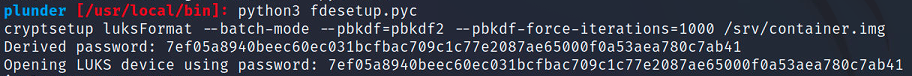
\includegraphics[width=1\textwidth]{img/fde_init_debug_output.png}
\end{center}
The image can be decrypted with:
\begin{lstlisting}[language=bash]
$ sudo cryptsetup luksOpen /srv/container.img container
\end{lstlisting}
The image can now be accessed with:
\begin{lstlisting}[language=bash]
$ sudo mount /dev/mapper/decrypted_devicess /media/my_device
\end{lstlisting}



\subsection*{Finding Details}
Using the ”ps aux” command the running processes on the \ac{DUT} can be determined. In the output of the command the following process can be seen (this is only a cutout of the output):
\begin{lstlisting}[language=bash]
root  965  0.0  0.9  16252  9188  Mar05   0:00 
/usr/bin/python3 /usr/local/bin/mgmtserver
\end{lstlisting}
This leads to the directory ”usr/local/bin” which contains the following files (outcut):
\begin{lstlisting}[language=bash]
$ ls -a
-rw------- 1 root root 4,0K 12.02.2023 18:52:59 check_version.pyc
-rwxr-xr-x 1 root root 4,2K 12.02.2023 19:14:51 c_rehash
-rwx------ 1 root root 4,0K 05.03.2023 11:14:51 fdesetup.pyc
-rwx------ 1 root root 2,5K 12.02.2023 19:58:22 mgmtserver
\end{lstlisting}
This is how the ”fdesetup.pyc” file can be discovered.
After searching on the \ac{DUT} for ”fdesetup.pyc” a service named ”fde\_init.service” can be discovered which lies in the directory ”/etc/systemd/system” and is used to execute the ”fdesetup.pyc” file.


The service looks like this:
\begin{lstlisting}[language=bash]
[Unit]
Description=FDE initialization
After=network-online.target

[Service]
Type=oneshot
ExecStart=/usr/bin/python3 /usr/local/bin/fdesetup.pyc
    
[Install]
WantedBy=multi-user.target
\end{lstlisting}
This service is always executed when the network of the \ac{DUT} is online.
The description indicates that this service is used for the encryption of the ”container.img” (FDE = Full Disk Encryption). The service also leads to the ”fdesetup.pyc” file. Trying to view the content of the python file results in mostly nonsense because the file is already compiled. But some buzzwords of the file can be seen like ”password” or ”luks”. The whole compiled ”fdesetup.pyc” file can be found in the appendix.
Not all decompilers are able to decompile the file due to the used python version. One decompiler that can be used is ”pycdc”.
The whole decompiled ”fdesetup.pyc” file can be found in the appendix.
To decrypt the configuration the following python scrpit was used:
\begin{lstlisting}[language=python]
#! /usr/bin/ python
from cryptography.fernet import Fernet
key = b'dGH1BR5gJ6wz6rneOkvmW50UsgY_J3kBZlRIUmsSiYw='

f = Fernet(key)

token =b'gAAAAAB6U1FZADONUKESIJFYDrY8jeRSFL2TqYpqfIiTrTP8ceG
BoffIZt7XvWS5pXWE9afjswEi_fSq9D-tcEnh8QflWQu2j4158VrbjbD1s8k
WRqcv665XHDiFSEDPAL1yb2w=='

decrypted f.decrypt(token)

print(decrypted)
\end{lstlisting}
Following is the decrypted default configuration used in the ”fdsetup.pyc” file:
\begin{lstlisting}[language=Bash]
"debug": false,
"initial_passphrase": "Q99mjPp4xMwnEpgJd4kd5LNe",
"mapper_name": "fde", 
"source_dev": "/srv/container.img", 
"interface_mac": "eth0",
"source_files": [
    ["/proc/cpuinfo", "filter_cpuinfo"], 
    ["/sys/kernel/debug/bluetooth/hci0/identity", null], 
    ["/sys/devices/platform/soc/3f980000.usb/usb1/1-1/1-1.1
/1-1.1:1.0/net/eth0/address", null]
]
\end{lstlisting}
This configuration also reveils the path to the encrypted image. The path is ”/srv/container.img”.


\subsection*{Evaluation of Results}
\begin{center}
    \begin{tabular}{cccc}
    \textbf{Effort to Fix:} & &\ \textbf{\textcolor{green!50!blue}{Low}}\
    \end{tabular}
\end{center}

The code shouldnt contain the debug option. Debugging can be used for development but should be removed before the code is used in production.
